\documentclass{article}
\usepackage[utf8]{inputenc}

\usepackage{amsmath}
\usepackage{float}
\usepackage{graphicx}
\usepackage{hyperref}
\hypersetup{
    colorlinks=true,
    linkcolor=black,
    filecolor=magenta,      
    urlcolor=blue,
}

\title{Machine Learning}
\author{Josh Myers-Dean \and Robin Cosbey}
\date{December 2019}

\begin{document}

\maketitle
\newpage
\tableofcontents
\newpage

\section{Introduction} 
The term ``machine learning'' was defined in 1959 as \textit{a field of study that gives computers the ability to learn without being explicitly programmed.} This means that rather than giving a computer a list of instructions to follow, we take advantage of the computer's representational abilities. The computer \textit{learns} patterns in data. Machine learning is essentially a math problem: $y = h(x)$ where $x$ is the input, $y$ is the output and $h$ represents the function (mathematical model) applied. In simple terms we are learning a mapping from $x$ to $y$. The goal of this workshop is to dive into the topics presented in \ref{fig:flow}, show how the process of each step and provide some resources.

\begin{figure}[H]
    \centering
    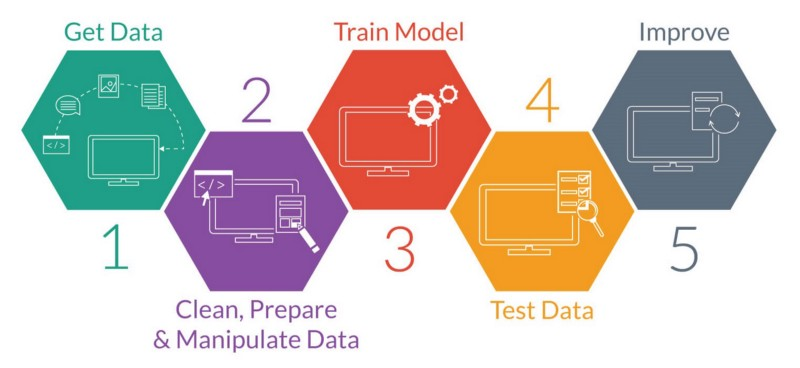
\includegraphics[width=3in]{flowchart.jpeg}
    \caption{General machine learning workflow. \href{https://www.freecodecamp.org/news/every-single-machine-learning-course-on-the-internet-ranked-by-your-reviews-3c4a7b8026c0/}{Link}}
    \label{fig:flow}
\end{figure}

\subsection{Unsupervised and Supervised Learning}
We primarily see \textit{unsupervised} and \textit{supervised} learning algorithms. Both are given a set of examples to learn from, known as \textit{training data}. In the case of supervised learning, we have ground truth output associated with the input data unlike unsupervised learning in which the computer is only given the input and ``clusters'' the examples based on similarity rather than learning from the mappings provided. Most of this workshop will focus on supervised learning. 
\begin{figure}[H]
    \centering
    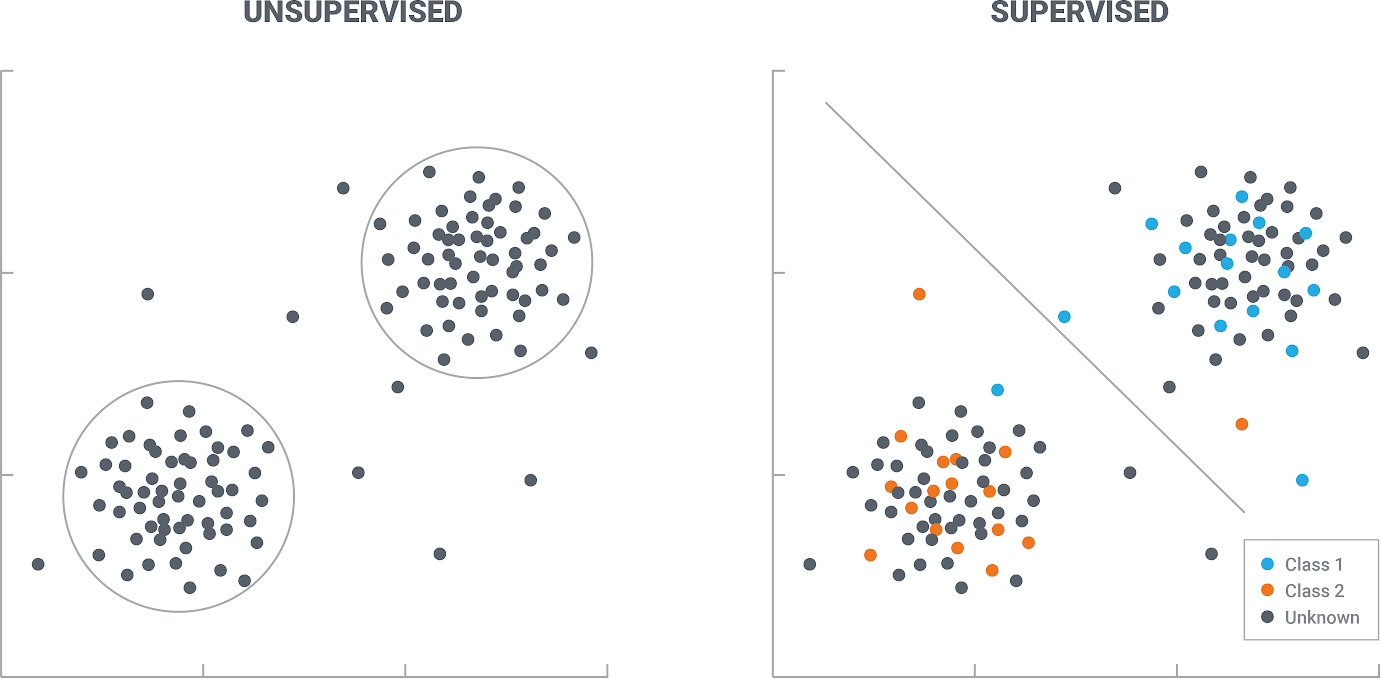
\includegraphics[width=3.1in]{supervision.png}
    \caption{Unsupervised consists of clustering whereas supervised (in this case binary classification) consists of finding a boundary between data points. \href{https://chatbotsmagazine.com/lets-know-supervised-and-unsupervised-in-an-easy-way-9168363e06ab}{Link}}
\end{figure}

\newpage
\subsection{Tasks} 

The two general types of problems that can be solved with supervised machine learning techniques are \textbf{classification} and \textbf{regression}. The main difference between the two is the output: classification has a categorical (discrete) output whereas regression has a numerical (continuous) output. 

\begin{figure}[H]
    \centering
    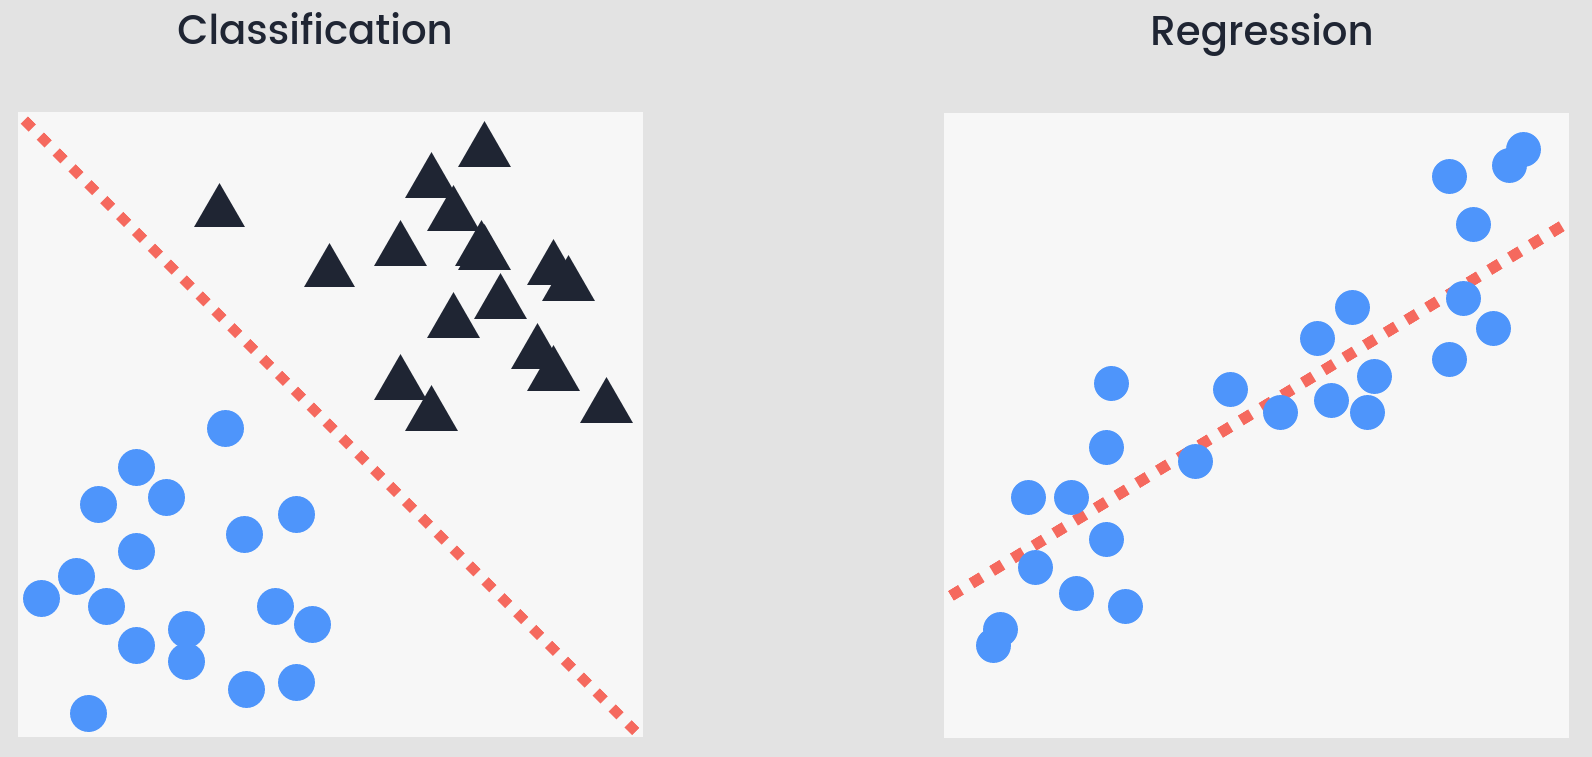
\includegraphics[width=3.5in]{tasks.png}
    \caption{Basic distinction between the two types of tasks. \href{https://medium.com/datadriveninvestor/supervised-vs-unsupervised-machine-learning-5200ffa7301a}{Link}}
    \label{fig:tasks}
\end{figure}

\subsubsection{Classification}
Classification algorithms are used when the outputs are restricted to a limited set of values. The basic form is \textit{binary classification} as shown in \ref{fig:tasks} in which the model assigns each input to one of two outputs. For example, if we have a model that identifies if an image contains a dog, the output would be the prediction of either `dog' or `not dog' (true or false).  

\begin{figure}[H]
    \centering
    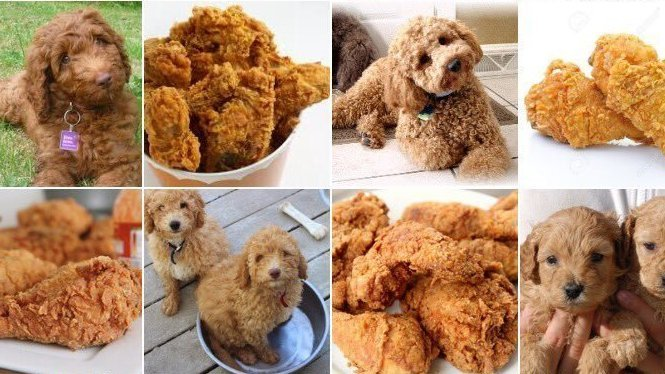
\includegraphics[width=3.5in]{dogs.jpg}
    \caption{Can you tell which photos contain a dog? Can a computer? \href{https://www.npr.org/sections/thesalt/2016/03/11/470084215/canine-or-cuisine-this-photo-meme-is-fetching}{Link}}
\end{figure}

\newpage
\subsubsection{Regression}
Regression involves continuous values such as temperature, length and price. You typically see regression models used for finding relationships between variables and for forecasting. How do age, gender and diet impact height? This is an example of input variables (age, gender and diet), referred to as \textit{predictor variables}, and their relationship to a single output (height) known as the \textit{outcome variable}. Unlike classification, we determine a trend from the training data fed into the model.  

\begin{figure}[H]
    \centering
    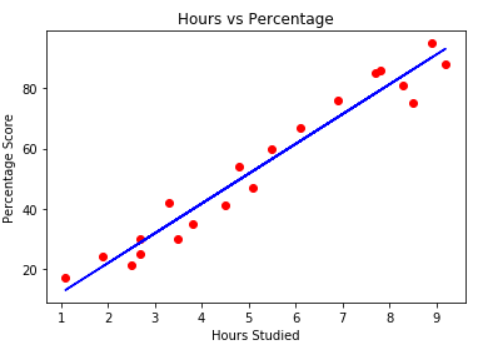
\includegraphics[width=3.5in]{regression.png}
    \caption{Regression line showing the relationship between hours studied and exam score. \href{https://stackabuse.com/linear-regression-in-python-with-scikit-learn/}{Link}}
\end{figure}

\newpage
\section{Data}
So what does data look like in machine learning? 
Aside from numerical data, anything that can be encoded as a numerical value or set of numerical values, such as images, words, or audio. 
With images, we can encode each pixel into their RGB numerical value. 
Audio data can be represented numerically based on features or by way of images with what are called spectograms. 
Words can be encoded as numbers, or word frequencies throughout an entire document might be used. 
We also use categorical data, a number that represents a group i.e. dogs, cats, or birds used primarily in classification tasks. 
Typically, this data is put into a matrix, let's examine some famous data sets where you can see real examples of data used in machine learning.

\subsection{Data Sets}
Let's examine some data sets that are commonly used by those exploring machine learning. Probably the most famous among these data sets, is the MNIST data set; a collection of handwritten numbers. We can use this data set to classify each picture as the number it is meant to represent. The MNIST data set is quite large and machine learning models are able to get up to 99\% accuracy classifying these images.

\begin{figure}[H]
    \centering
    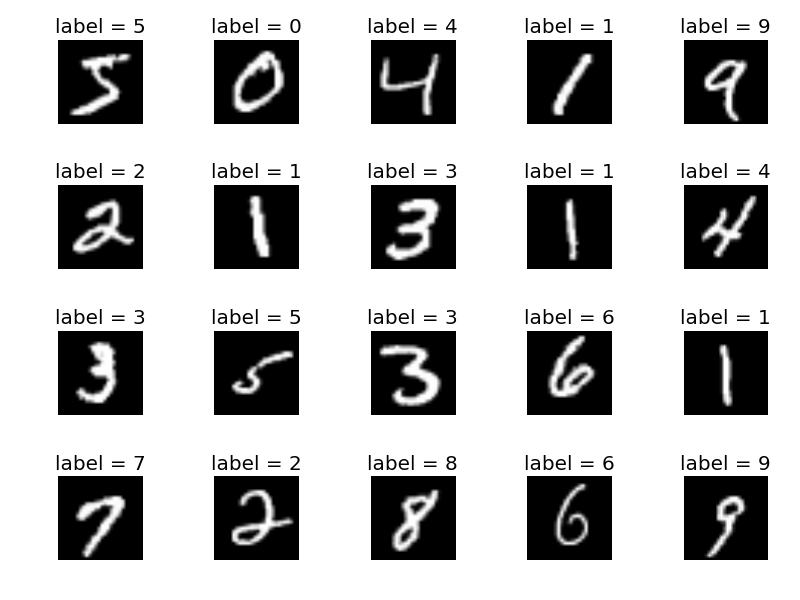
\includegraphics[width=4.5in]{mnist.png}
    \caption{MNIST Data set \href{http://yann.lecun.com/exdb/mnist/}{dataset linked here}.}
\end{figure}

\newpage

Another smaller data set is the Iris data set. In this case, we are not dealing with image data, we are given attributes. There are three kinds of iris represented in this data set and we are given four attributes of each flower: the sepal length and width, and the petal length and width.  

\begin{figure}[H]
    \centering
    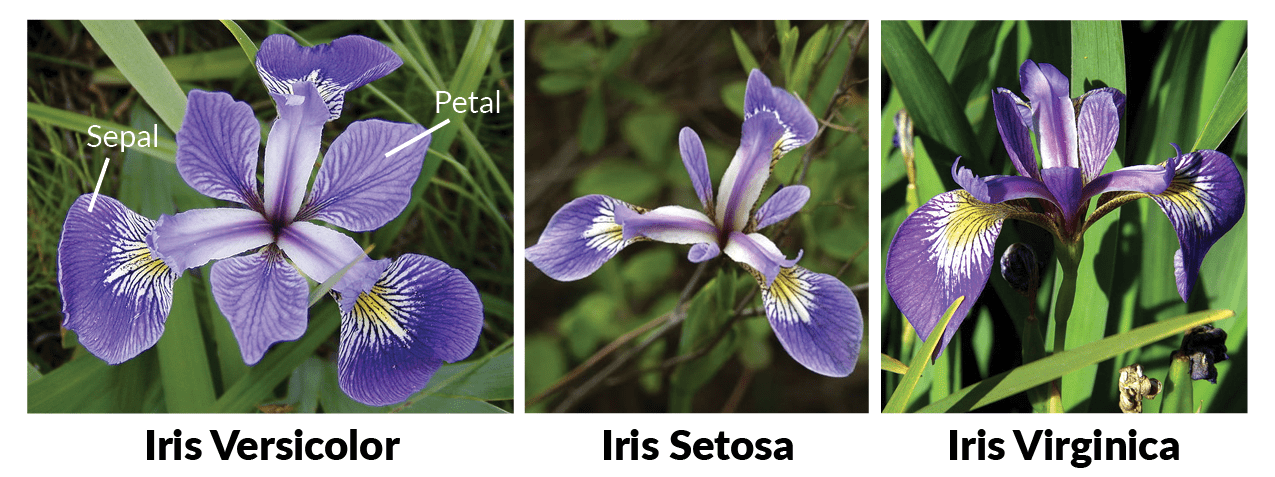
\includegraphics[width=4.5in]{iris.png}
    \caption{Iris Data set \href{https://archive.ics.uci.edu/ml/datasets/iris}{dataset linked here}.}
\end{figure}

This is a great data set for beginners because there are only 150 iris samples, making it easy to test and debug. Take a look at the links included to get a feel for what data looks like in machine learning.

\subsection{Bias in Data}
As you begin a machine learning project, one of the first steps is to find the dataset you will be working with. As you are forming the initial questions that you hope to answer with your efforts make sure to also ask the data some questions. Before you start building a model to work with the data, you should have a firm understanding of the distribution and makeup of the data itself. Many news stories have surfaced over the years indicating the explicit, inherent biases in many publicly released face and object recognition systems and it is not hard to believe that similar stories can be found in other domains. 

This analysis of your data is especially important when considering problems directly related to society. As the systems we build gain trust from the public, we, as computer scientists, can have great implications unknowingly on the world we live in. Throughout this analysis be on the lookout for an uneven distribution of data. Additionally, keep in mind that the biases present throughout history can be found implicitly in the datasets produced in those times and by using that data to train a model you are propagating those biases forward through time. Sometimes you may need to evaluate the types of problems you are looking to solve and ensure the value of this pursuit for the community.

\newpage
\subsection{Data Preparation}
The above datasets, MNIST and Iris, are \textit{clean}. There are no missing values, or random Unicode characters that are going to trip you up when trying to parse the data. Often, data needs to be cleaned and made consistent. This process of making sure that data is clean can take up a lot of time. If an entire chunk of data is missing should it be averaged with its neighbors or be given the value of the previous data point? These are considerations a machine learning engineer will encounter. There is also the consideration of how to store input and output data as you will often train and re-train a model many times with different parameters that can be tuned called hyperparameters or maybe parse the data in a different way to see if that leads to any performance gains. Since you will want to run your model many times, you don't want to have to re-parse your cleaned data each time you want to run it as that takes a lot of time, so you will want to store your cleaned data somehow. You may also want to save various configurations of your trained model, so you will need an efficient and organized way to store trained models. You can also create data based off of your current data set, this is called data augmentation and may be something as simple as when building an image classifier reflecting some of your images horizontally or vertically to make you model more robust to image orientation. So, data preparation is a complex beast. There are many techniques that can be explored and many components to consider when preparing data.

After our data has been cleaned we typically want to split our data into train, development (sometimes called ``validation''), and test. You'll understand more in depth as to how these data sets are used after reading the \textit{Training} section. For now, understand that in order to train a model we will need data it can see (train), new data it can see to check its progress while training (development), and more data to see if it learned a pattern that can be applied to unseen data (test). We generally want to reserve 70\% for our training set, 10\% for our development set, and 20\% for our test set. You are not limited to splitting your data in this way and can try out different configurations as well.

\subsection{Training} 
Once we have an understanding of the data we are working with, have preprocessed the data appropriately and split the data into a train, development and test set, now it is time to design your model. More on the types of the basic machine learning and deep learning models in future sections. The training phase allows the the model to learn from the examples provided and understand the presents in the data. The development, or validation, phase is when we tune hyperparameters -- \textit{hyperparameters} are typically related to the model architecture. Slight changes to the hyperparameters will produce different results with the model. This process repeats for a predefined amount of time. Only once we have completed training and hyperparameter tuning do we turn to the test data. The test set is used to independently assess the accuracy of the model on held out data that has not been seen previously. 

\newpage
\section{Machine Learning \& Deep Learning} 
There are many differences between deep learning and machine learning algorithms. Features are pieces of information that are intended to be relevant to performing a task. For example, if we were to build an animal classifier using a machine learning algorithm a feature we may want to include is the type of coat an animal has: fur, scales, or feathers. We would want to include as many of these distinctive features as possible for each animal and then give those pieces of information to our machine learning algorithm and this would create a model that can classify animals. But with deep learning we wouldn't need to manually identify distinctive characteristics of animals, we can just give our deep learning algorithm thousands of pictures of animals. Deep learning algorithms are capable of finding which pieces of information about a picture for example, are important without human assistance. This is one benefit of deep learning algorithms.

Another difference between machine learning and deep learning algorithms is their expressiveness. Machine learning algorithms generally revolve around optimizing linear functions to fit our data. However, not all patterns found in data can be expressed by linear functions. 

\begin{figure}[H]
    \centering
    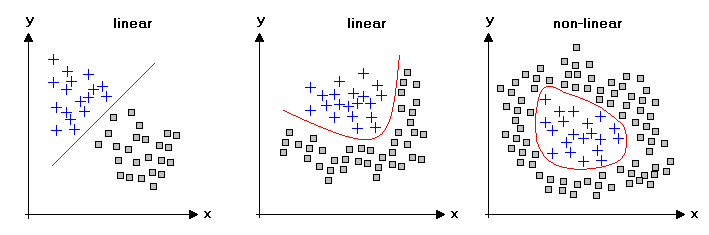
\includegraphics[width=5.0in]{linearvsnonlinear.png}
    \caption{Non-linear models are able to model more complex patterns.}
\end{figure}

Deep learning algorithms can consist of one or more linear or non-linear transformations. Because of this, deep learning models are able to model both linear and non-linear patterns in data. This is very powerful, and is the \textit{secret sauce} of deep learning models. Because deep learning algorithms are able to model much more complex and nuanced patterns in data, they require a lot more data than traditional machine learning algorithms which are trying to model simpler patterns. While a machine learning model may require thousands of data points to do well, a deep learning model may require millions making deep learning much more computationally expensive.

\newpage
\subsection{Decision Trees} 
Decision trees are tree-like structures that can represent probability, decisions, and much more.

\begin{figure}[H]
    \centering
    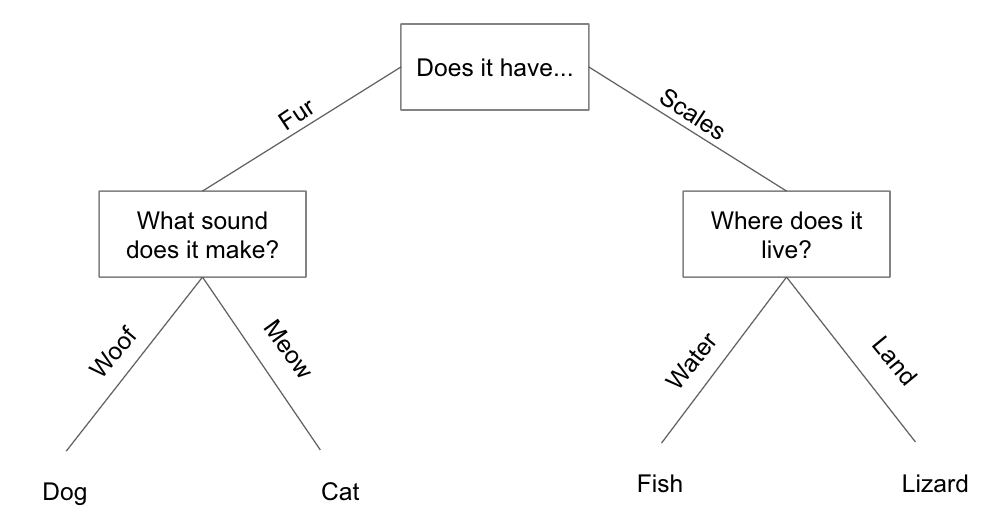
\includegraphics[width=4.5in]{decisiontree.png}
    \caption{Decision Tree}
\end{figure}

\subsubsection{Random Forest}
Random Forest is a supervised machine learning algorithm that can be used for both classification and regression tasks that consists of a collection of decision trees, hence the name. Here is the general algorithm:

\begin{enumerate}
    \item Split data into $n$ random sets selecting $m$ random features from each sample.
    \item Create a decision tree using each subset of data.
    \item Given new sample, each of these independent trees makes a prediction.
    \item The prediction with the most "votes" from our trees is our overall prediction.
\end{enumerate}

For a regression task, we would average the predictions made by all of the decision trees. This idea of averaging decisions of multiple models is called bootstrap aggregating or bagging and can reduce variance and overfitting.

Essentially, every decision tree will make a prediction and the most common prediction in among all of the decision trees will be the outcome. When using the random forest algorithm for regression, we will average the output of each decision tree. 

\newpage
\subsection{Support Vector Machines (SVMs)} 
Support vector machines are a simple model that do not require a large amount of data and separate classes represented in data. SVMs are simple discriminative classifiers that output an optimal decision boundary between the datapoints provided. When new datapoints are fed through the SVM, they are classified based on where they fall in relation to the decision boundary. This boundary is often referred to as a ``hyperplane.''  The margin is the distance from the boundary to the nearest datapoint. We want to find a decision boundary that allows points to be in their respective classes without crossing the boundary into other classes and a good margin is one where this separation is large for all classes represented. scikit-learn offers a SVM tool that is easy to download to test with given data. More information about SVMs and the toolkit can be found \href{https://scikit-learn.org/stable/modules/svm.html}{here}.

\begin{figure}[H]
    \centering
    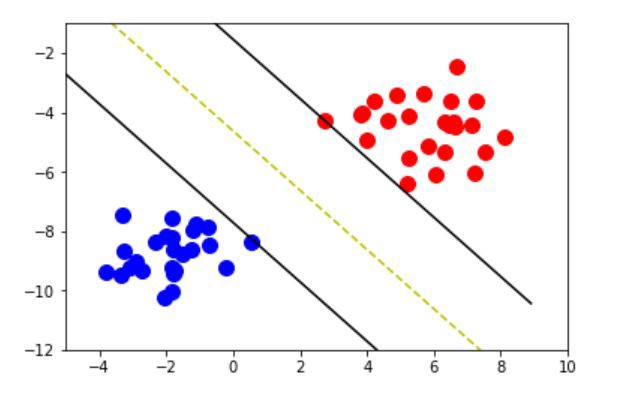
\includegraphics[width=3.5in]{svm.jpeg}
    \caption{Decision boundary (yellow dashed line) separating the red from blue. \href{https://medium.com/deep-math-machine-learning-ai/chapter-3-support-vector-machine-with-math-47d6193c82be}{Link}}
\end{figure}

\newpage
\subsection{KNN} 
K-Nearest Neighbors is an supervised machine learning algorithm that can be used for classification and regression tasks. Let's focus on classification. In this case we won't do any training using our training data, we will using the position of our training data in space to classify unseen data points.

\begin{figure}[H]
    \centering
    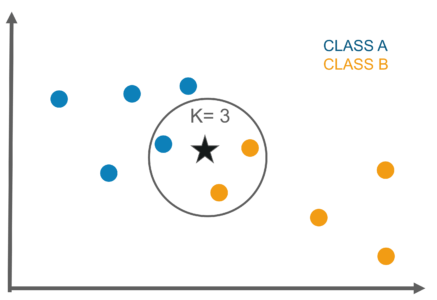
\includegraphics[width=4.0in]{knn.png}
    \caption{KNN Algorithm.}
\end{figure}

\begin{enumerate}
    \item Select number of neighbors to examine $k$.
    \item Given an unseen data point, find $k$ nearest data points.
    \item The class that appears the most of those $k$ nearest data points is the class of our unseen data point.
\end{enumerate}

You can experiment with different distance metrics like Euclidean distance, Manhattan distance, or Cosine similarity. Because there is no training time involved, this can be a good option when time is limited and is relatively easy to setup. K-Nearest Neighbors may not be a good idea if you have very high dimensional or feature-rich data. This is because of something called the Curse of Dimensionality; as we go into higher and higher dimensional space distance as we know it becomes more skewed and two things that are very different may seem to be "close" to each other in high dimensional space. For more on the Curse of Dimensionality and how higher dimensionality can affect your models read \href{https://towardsdatascience.com/curse-of-dimensionality-2092410f3d27}{this article}.

\newpage
\subsection{Deep Neural Networks (DNNs)} 
DNNs are commonly used within problem spaces with a lot of available data. Once the data is preprocessed, we provide the data as input to the DNN. The data undergoes a series of non-linear transformations. This is what separates deep neural networks from one-layer, shallow, linear neural networks. These transformations are followed by a linear transformation which produces the output or result. 
\begin{figure}[H]
    \centering
    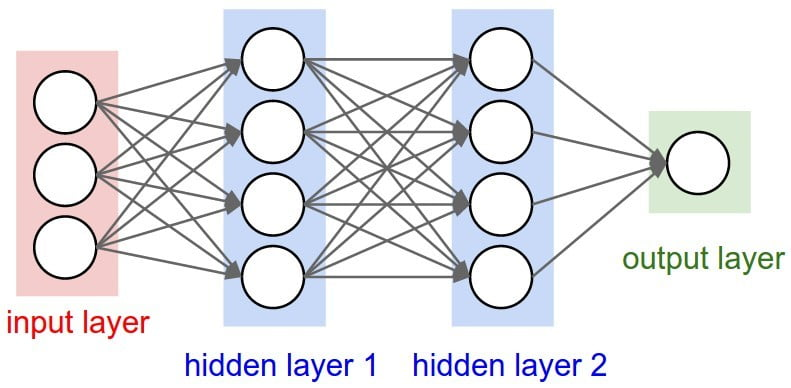
\includegraphics[width=3.5in]{nn.jpg}
    \caption{Simple DNN with two hidden non-linear layers. \href{https://www.digitaltrends.com/cool-tech/what-is-an-artificial-neural-network/}{Link}}
\end{figure}

\href{https://playground.tensorflow.org}{Tutorial here.}

\newpage
\subsection{Convolutional Neural Networks (CNNs)} 

Convolutional Neural Networks are mostly used with image data to perform image classification and other image related tasks.

\begin{figure}[H]
    \centering
    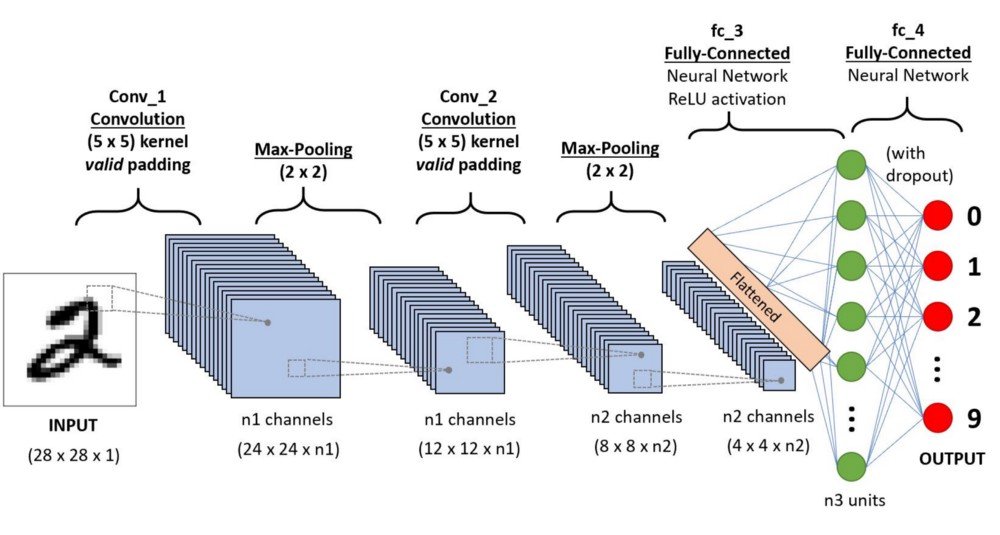
\includegraphics[width=4.5in]{cnn.jpeg}
    \caption{Unrolling an RNN. Each input is fed through to produce an output at the given timestep. We also pass context forward through time. \href{https://towardsdatascience.com/a-comprehensive-guide-to-convolutional-neural-networks-the-eli5-way-3bd2b1164a53}{Link}}
\end{figure}

\subsection{Recurrent Neural Networks (RNNs)} 

Recurrent Neural Networks strength lies in finding patterns in sequential data, whether that be sentences, audio, or protein sequences. They have special cells which allow them to keep important information seen from past samples or from future samples. There are many different variations of RNNs, here is a link to some RNN tutorials written in PyTorch \href{https://github.com/yunjey/pytorch-tutorial/tree/master/tutorials/02-intermediate}{here}.

\begin{figure}[H]
    \centering
    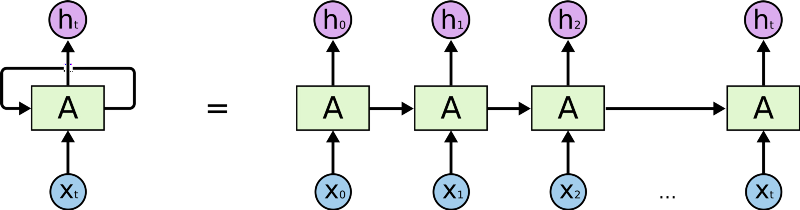
\includegraphics[width=4.5in]{rnn.png}
    \caption{Unrolling an RNN. Each input is fed through to produce an output at the given timestep. We also pass context forward through time. \href{https://medium.com/@jianqiangma/all-about-recurrent-neural-networks-9e5ae2936f6e}{Link}}
\end{figure}

\newpage
\section{Further Topics}

\subsection{Reinforcement Learning}
\href{https://deepmind.com/research/publications/playing-atari-deep-reinforcement-learning/}{Paper}
\begin{figure}[H]
    \centering
    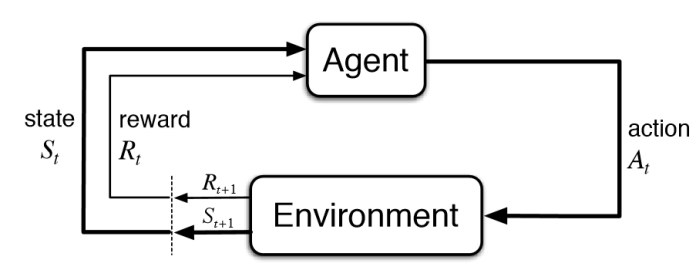
\includegraphics[width=4.5in]{rl.jpg}
    \caption{In recent years deep learning has been introduced to reinforcement learning algorithms to improve performance. The agent chooses an action and receives updated information of the environment in order to choose a new action. Deep approaches have been used to augment the agent. \href{https://www.kdnuggets.com/2018/03/5-things-reinforcement-learning.html}{Link}}
\end{figure}

\subsection{Generative Adversarial Networks}
\href{https://arxiv.org/abs/1406.2661}{Paper}
\begin{figure}[H]
    \centering
    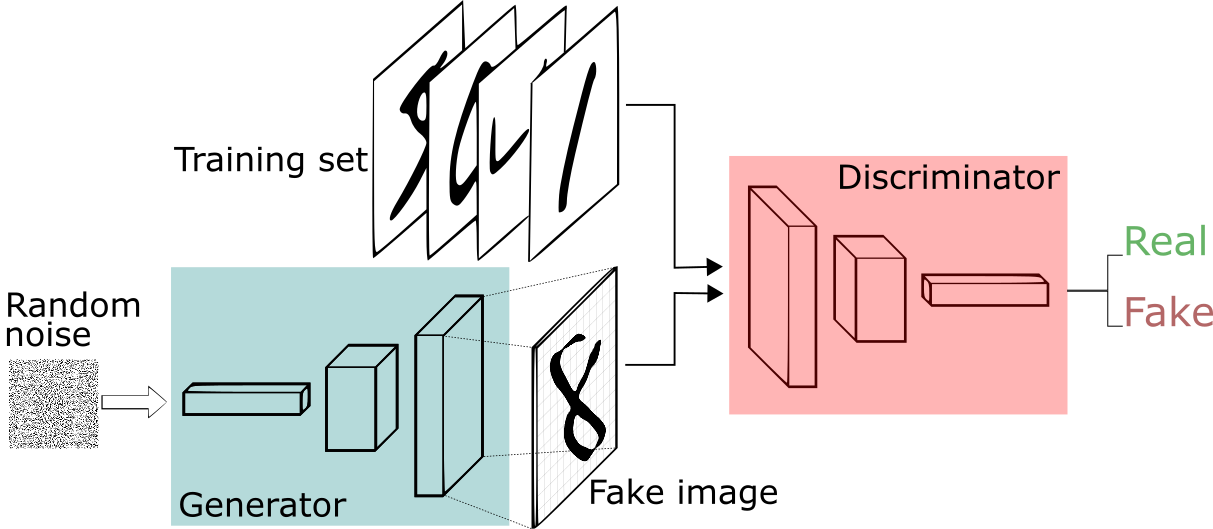
\includegraphics[width=4.5in]{gans.png}
    \caption{We have been able to achieve incredible results using this model to generate things. This is done by training a generator and discriminator model. The generator tries to generate a realistic sample from the training set and the discriminator does its best to tell if the sample given to it is from the training set or a generated "fake" sample. By doing this we are able to train a generator that can create extremely good "fakes" or generated samples. Things it may try to "fake" and generate are images, audio, or video. \href{https://skymind.ai/wiki/generative-adversarial-network-gan}{Link}}
\end{figure}

\newpage
\subsection{Few Shot Learning}
\href{https://openreview.net/forum?id=HkxLXnAcFQ}{Paper}
\begin{figure}[H]
    \centering
    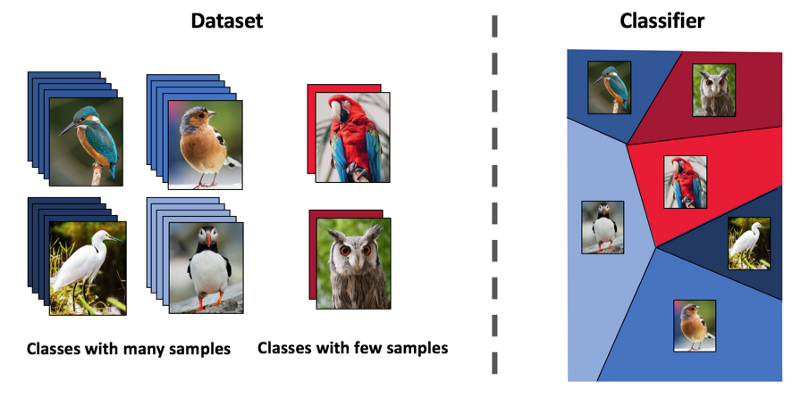
\includegraphics[width=4.5in]{fewshot.png}
    \caption{Few shot learning works to train a model on very few examples of given classes. Many training episodes are used to understand the distinctions between the classes provided.  \href{https://medium.com/sap-machine-learning-research/deep-few-shot-learning-a1caa289f18}{Link}}
\end{figure}

\newpage
\section{Resources}


\end{document}
